\chapter{\sffamily Building a generalised simulator}

{\bfseries\sffamily Concept.} To design and build a generalised simulation engine that is able to generate samples from a `Pokédex' of possible stochastic processes that a researcher might encounter. A `Pokédex' here is just a fanciful description for a very general class of multidimensional stochastic processes that pop up everywhere in taming the mathematical wilds of real-world phenomena, and which also leads to a name for the software itself: the `stochadex'. With such a thing pre-built and self-contained, it can become the basis upon which to build generalised software solutions for a lot of different problems. For the mathematically-inclined, this chapter will require the introduction of a new formalism which we shall refer back to throughout the book. For the programmers, the public Git repository for the code that is described in this chapter can be found here: \href{https://github.com/umbralcalc/stochadex}{https://github.com/umbralcalc/stochadex}.

\section{\sffamily Computational formalism}

Before we dive into software design of the stochadex, we need to mathematically define the general computational approach that we're going to take. Because the language of stochastic processes is primarily mathematics, we'd argue this step is essential in enabling a really general description. From experience, it seems reasonable to start by writing down the following formula which describes iterating some arbitrary process forward in time (by one finite step) and adding a new row each to some matrix $X' \rightarrow X$
%%
\begin{align}
X^{i}_{{\sf t}+1} &= F^{i}_{{\sf t}+1}(X',z,{\sf t}) \,, \label{eq:x-step-def}
\end{align}
%%
where: $i$ is an index for the dimensions of the `state' space; ${\sf t}$ is the current time index for either a discrete-time process or some discrete approximation to a continuous-time process; $X$ is the next version of $X'$ after one timestep (and hence one new row has been added); $z$ is a vector of arbitrary size which contains the `hidden' other parameters that are necessary to iterate the process; and $F^i_{{\sf t}+1}(X',z,{\sf t})$ as the latest element of an arbitrary matrix-valued function. As we shall discuss shortly, $F^i_{{\sf t}+1}(X',z,{\sf t})$ may represent not just operations on deterministic variables, but also on stochastic ones. There is also no requirement for the function to be continuous.

\begin{figure}[h]
\centering
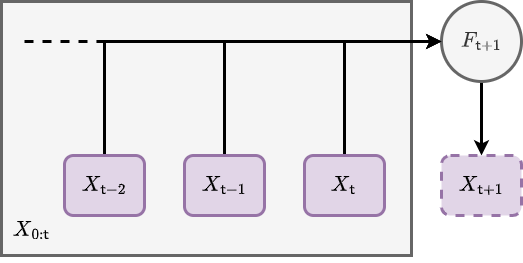
\includegraphics[width=10cm]{images/chapter-1-fundamental-loop.drawio.png}
\caption{Graph representation of Eq.~(\ref{eq:x-step-def}).}
\label{fig:fundamental-loop}
\end{figure}

The basic computational idea here is illustrated in Fig.~\ref{fig:fundamental-loop}; we iterate the matrix $X$ forward in time by a row, and use its previous version $X'$ as an entire matrix input into a function which populates the elements of its latest rows. In pseudocode you could easily write something with the same idea in it, and it would probably look something like the method diagram in Fig.~\ref{fig:fundamental-loop-code}.

\begin{figure}[h]
\centering
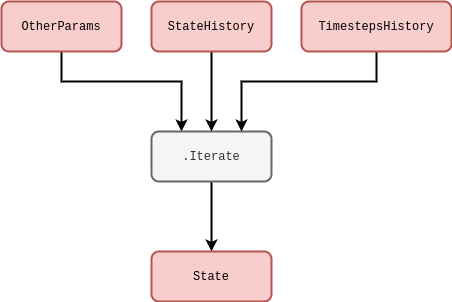
\includegraphics[width=10cm]{images/chapter-1-fundamental-loop-code.drawio.png}
\caption{Pseudocode representation of Eq.~(\ref{eq:x-step-def}).}
\label{fig:fundamental-loop-code}
\end{figure}

Pretty simple! But why go to all this trouble of storing matrix inputs for previous values of the same process? It's true that this is mostly redundant for \emph{Markovian} phenomena, i.e., processes where their only memory of their history is the most recent value they took. However, for a large class of stochastic processes a full memory\footnote{Or memory at least within some window.} of past values is essential to consistently construct the sample paths moving forward. This is true in particular for \emph{non-Markovian} phenomena, where the latest values don't just depend on the immediately previous ones but can depend on values which occured much earlier in the process as well.

For more complex physical models and integrators, the distinct notions of `numerical timestep' and `total elapsed continuous time' will crop up quite frequently. Hence, before moving on further details, it will be important to define the total elapsed time variable $t({\sf t})$ for processes which are defined in continuous time. Assuming that we have already defined some function $\delta t({\sf t})$ which returns the specific change in continuous time that corresponds to the step ${\sf t}-1 \rightarrow {\sf t}$, we will always be able to compute the total elapsed time through the relation
%%
\begin{align}
t({\sf t}) &= \sum^{{\sf t}}_{{\sf t}'=0}\delta t({\sf t}') \label{eq:t-steps-sum} \,.
\end{align}
%%
This seems a lot of effort, no? Well it's important to remember that our steps in continuous time may not be constant, so by defining the $\delta t({\sf t})$ function and summing over it we can enable this flexibility in the computation. In case the summation notation is no fun for programmers; we're simply adding up all of the differences in time to get a total. We've illustrated this in Fig.~\ref{fig:time-step-summation} for more clarity.

\begin{figure}[h]
\centering
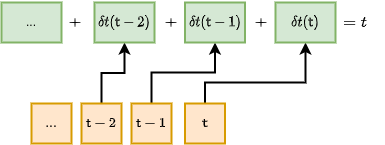
\includegraphics[width=10cm]{images/chapter-1-time-step-summation.drawio.png}
\caption{Illustration of Eq.~(\ref{eq:t-steps-sum}).}
\label{fig:time-step-summation}
\end{figure}

So, now that we've mathematically defined a really general notion of iterating the stochastic process forward in time, it makes sense to discuss some simple examples. For instance, it is frequently possible to split $F$ up into deteministic (denoted $D$) and stochastic (denoted $S$) matrix-valued functions like so
%%
\begin{align}
& F^{i}_{{\sf t}+1}(X',z,{\sf t}) = D^{i}_{{\sf t}+1}(X',z,{\sf t}) + S^{i}_{{\sf t}+1}(X',z,{\sf t}) \,.
\end{align}
%%
In the case of stochastic processes with continuous sample paths, it's also nearly always the case with mathematical models of real-world systems that the deterministic part will at least contain the term $D^{i}_{{\sf t}+1}(X',z,{\sf t}) = X^i_{\sf t}$ because the overall system is described by some stochastic differential equation. This is not a really requirement in our general formalism, however.

What about the stochastic term? For example, if we wanted to consider a \emph{Wiener process noise}, we can define $W^i_{{\sf t}}$ is a sample from a Wiener process for each of the state dimensions indexed by $i$ and our formalism becomes
%%
\begin{align}
& S^{i}_{{\sf t}+1}(X',z,{\sf t}) = W^i_{{\sf t}+1}-W^i_{\sf t} \label{eq:wiener}\,.
\end{align}
%%
One draws the increments $W^i_{{\sf t}+1}-W^i_{\sf t}$ from a normal distribution with a mean of $0$ and a variance equal to the length of continuous time that the step corresponded to $\delta t({\sf t}+1)$, i.e., the probability density $P^i_{{\sf t}+1}(x)$ of the increments $x^i=W^i_{{\sf t}+1}-W^i_{\sf t}$ is
%%
\begin{align}
P^i_{{\sf t}+1}(x) &= {\sf NormalPDF}[x^i;0,\delta t({\sf t}+1)] \,.
\end{align}
%%
Note that for state spaces with dimensions $>1$, we could also allow for non-trivial cross-correlations between the noises in each dimension. In pseudocode, the Wiener process is schematically represented by Fig.~\ref{fig:wiener-process}.

\begin{figure}[h]
\centering
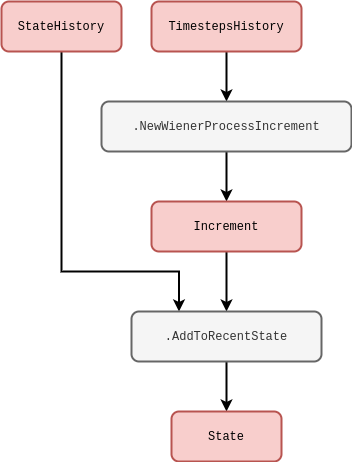
\includegraphics[width=8cm]{images/chapter-1-wiener-process.drawio.png}
\caption{Schematic of code for a Wiener process.}
\label{fig:wiener-process}
\end{figure}

In another example, to model \emph{geometric Brownian motion noise} we would simply have to multiply $X^i_{\sf t}$ to the Wiener process like so
%%
\begin{align}
& S^{i}_{{\sf t}+1}(X',z,{\sf t}) = X^i_{\sf t}(W^i_{{\sf t}+1}-W^i_{\sf t})\label{eq:gbm} \,.
\end{align}
%%
Here we have implicitly adopted the Itô interpretation to describe this stochastic integration. Given a carefully-defined integration scheme other interpretations of the noise would also be possible with our formalism too, e.g., Stratonovich\footnote{Which would implictly give $S^{i}_{{\sf t}+1}(X',z,{\sf t}) = (X^i_{{\sf t}+1}+X^i_{\sf t})(W^i_{{\sf t}+1}-W^i_{\sf t}) / 2$ for Eq.~(\ref{eq:gbm}).} or others within the more general `$\alpha$-family'~\cite{van1992stochastic,risken1996fokker,rog-will-2000}. The pseudocode for any of these should hoepfully be fairly straightforward to deduce based on the lines we've already written above.

\begin{figure}[h]
\centering
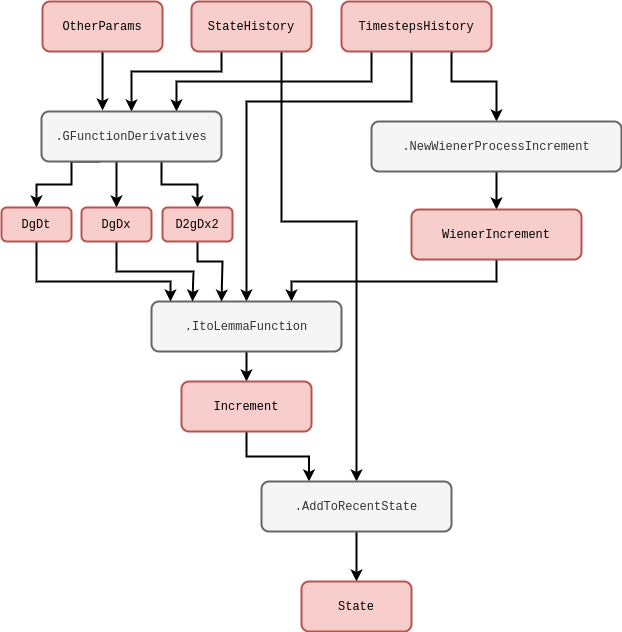
\includegraphics[width=12cm]{images/chapter-1-ito-lemma.drawio.png}
\caption{Schematic of code for Eq.~(\ref{eq:general-wiener}).}
\label{fig:ito-lemma}
\end{figure}

We can imagine even more general processes that are still Markovian. One example of these in a single-dimension state space would be to define the noise through some general function of the Wiener process like so
%%
\begin{align}
S^0_{{\sf t}+1}(X',z,{\sf t}) &= g[W^0_{{\sf t}+1},t({\sf t}+1)]-g[W^0_{\sf t}, t({\sf t})] \\
&= \bigg[ \frac{\partial g}{\partial t} + \frac{1}{2}\frac{\partial^2 g}{\partial x^2} \bigg] \delta t ({\sf t}+1) + \frac{\partial g}{\partial x} (W^0_{{\sf t}+1}-W^0_{\sf t}) \label{eq:general-wiener}\,,
\end{align}
%%
where $g(x,t)$ is some continuous function of its arguments which has been expanded out with Itô's Lemma on the second line. Note also that the computations in Eq.~(\ref{eq:general-wiener}) could be performed with numerical derivatives in principle, even if the function were extremely complicated. This is unlikely to be the best way to describe the process of interest, however, the mathematical expressions above can still be made a bit more meaningful to the programmer in this way. The pseudocode in general would look something like Fig.~\ref{fig:ito-lemma}.

Let's now look at a more complicated type of noise. For example, we might consider sampling from a \emph{fractional Brownian motion} process $[B_{H}]_{\sf t}$, where $H$ is known as the `Hurst exponent'. Following Ref.~\cite{decreusefond1999stochastic}, we can simulate this process in one of our state space dimensions by modifying the standard Wiener process by a fairly complicated integral factor which looks like this
%%
\begin{align}
S^{0}_{{\sf t}+1}(X',z,{\sf t}) &= \frac{(W^0_{{\sf t}+1} - W^0_{\sf t})}{\delta t({\sf t})}\int^{t({\sf t}+1)}_{t({\sf t})}{\rm d}t' \frac{(t'-t)^{H-\frac{1}{2}}}{\Gamma (H+\frac{1}{2})} {}_2F_1 \bigg( H-\frac{1}{2};\frac{1}{2}-H;H+\frac{1}{2};1-\frac{t'}{t}\bigg) \label{eq:fbm} \,,
\end{align}
%%
where $S^{0}_{{\sf t}+1}(X',z,{\sf t})=[B_{H}]_{{\sf t}+1}-[B_{H}]_{{\sf t}}$. The integral in Eq.~(\ref{eq:fbm}) can be approximated using an appropriate numerical procedure (like the trapezium rule, for instance). In the expression above, we have used the symbols ${}_2F_1$ and $\Gamma$ to denote the ordinary hypergeometric and gamma functions, respectively. A computational form of this integral is illustrated in Fig.~\ref{fig:fractional-brownian-motion} to try and disentangle some of the mathematics as a program.

\begin{figure}[h]
\centering
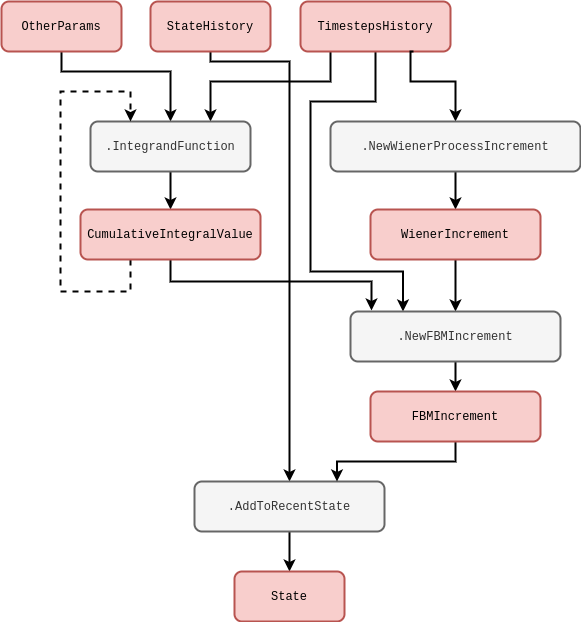
\includegraphics[width=11cm]{images/chapter-1-fractional-brownian-motion.drawio.png}
\caption{Schematic of code for Eq.~(\ref{eq:fbm}).}
\label{fig:fractional-brownian-motion}
\end{figure}

So far we have mostly been discussing noises with continuous sample paths, but we can easily adapt our computation to discontinuous sample paths as well. For instance, \emph{Poisson process noises} would generally take the form
%%
\begin{align}
S^{i}_{{\sf t}+1}(X',z,{\sf t}) &= [N_{\lambda}]^i_{{\sf t}+1}-[N_{\lambda}]^i_{\sf t}\,,
\end{align}
%%
where $[N_{\lambda}]^i_{\sf t}$ is a sample from a Poisson process with rate $\lambda$. One can think of this process as counting the number of events which have occured up to the given interval of time, where the intervals between each succesive event are exponentially distributed with mean $1/\lambda$. Such a simple counting process could be simulated exactly by explicitly setting a newly-drawn exponential variate to the next continuous time jump ${\delta t}({\sf t}+1)$ and iterating the counter. Other exact methods exist to handle more complicated processes involving more than one type of `event', such as the Gillespie algorithm~\cite{gillespie1977exact} --- though these techniques are not always be applicable in every situation.

Is using step size variation always possible? If we consider a \emph{time-inhomogeneous Poisson process noise}, which would generally take the form
%%
\begin{align}
S^{i}_{{\sf t}+1}(X',z,{\sf t}) &= [N_{\lambda ({\sf t}+1)}]^i_{{\sf t}+1}-[N_{\lambda ({\sf t})}]^i_{\sf t}\,,
\end{align}
%%
the rate $\lambda ({\sf t})$ has become a deterministically-varying function in time. In this instance, it likely not be accurate to simulate this process by drawing exponential intervals with a mean of $1/\lambda ({\sf t})$ because this mean could have changed by the end of the interval which was drawn. An alternative approach (which is more generally capable of simulating jump processes but is an approximation) first uses a small time interval $\tau$ such that the most likely thing to happen in this period is nothing, and then the probability of the event occuring is simply given by
%%
\begin{align}
p({\sf event}) &= \frac{\lambda ({\sf t})}{\lambda ({\sf t}) + \frac{1}{\tau}} \label{eq:rejection}\,.
\end{align}
%%
This idea can be applied to phenomena with an arbitrary number of events and works well as a generalised approach to event-based simulation, though its main limitation is worth remembering; in order to make the approximation good, $\tau$ often must be quite small and hence our simulator must churn through a lot of steps. From now on we'll refer to this well-known technique as the \emph{rejection method}. Fig.~\ref{fig:inhomogeneous-poisson} may also help to understand this concept from the programmer's perspective.

\begin{figure}[h]
\centering
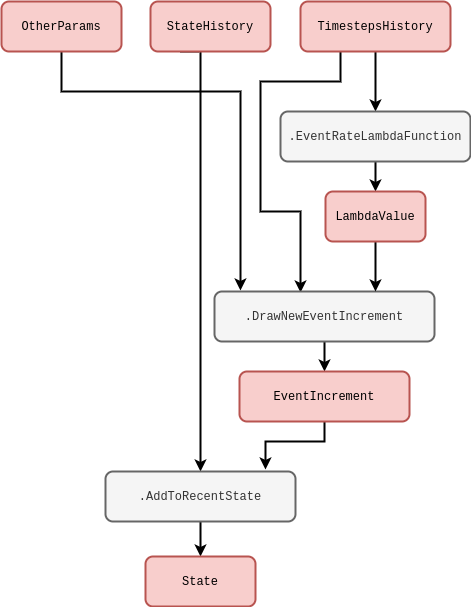
\includegraphics[width=9cm]{images/chapter-1-inhomogeneous-poisson.drawio.png}
\caption{Schematic of code for an inhomogeneous Poisson process.}
\label{fig:inhomogeneous-poisson}
\end{figure}

There are a few extensions to the simple Poisson process that introduce additional stochastic processes. \emph{Cox (doubly-stochastic) processes}, for instance, are basically where we replace the time-dependent rate $\lambda ({\sf t})$ with independent samples from some other stochastic process $\Lambda ({\sf t})$. For example, a Neyman-Scott process~\cite{neyman1958statistical} can be mapped as a special case of this because it uses a Poisson process on top of another Poisson process to create maps of spatially-distributed points. In our formalism, a two-state implementation of the Cox process noise would look like
%%
\begin{align}
S^{0}_{{\sf t}+1}(X',z,{\sf t}) &= \Lambda ({\sf t}+1) \\
S^{1}_{{\sf t}+1}(X',z,{\sf t}) &= [N_{S^{0}_{{\sf t}+1}}]^i_{{\sf t}+1}-[N_{S^{0}_{{\sf t}}}]^i_{\sf t}\,.
\end{align}
%%
This process could be simulated using the pseudocode we wrote for the time-inhomogeneous Poisson process previously --- where we would just replace \texttt{EventRateLambdaFunction} with a function that generates the stochastic rate $\Lambda ({\sf t})$.

Another extension is \emph{compound Poisson process noise}, where it's the count values $[N_{\lambda}]^i_{\sf t}$ which are replaced by independent samples $[J_{\lambda}]^i_{\sf t}$ from another probability distribution, i.e.,
%%
\begin{align}
S^{i}_{{\sf t}+1}(X',z,{\sf t}) &= [J_{\lambda}]^i_{{\sf t}+1}-[J_{\lambda}]^i_{\sf t}\,.
\end{align}
%%
Note that the rejection method of Eq.~(\ref{eq:rejection}) can be employed effectively to simulate any of these extensions as long as a sufficiently small $\tau$ is chosen. Once again, the pseudocode we wrote previously would be sufficient to simulate this process with one tweak: add into the \texttt{DrawNewEventIncrement} function the calling of a function which generates the $[J_{\lambda}]^i_{\sf t}$ samples and output these if the event occurs.

All of the examples we have discussed so far are Markovian. Given that we have explicitly constructed the formalism to handle non-Markovian phenomena as well, it would be worthwhile going some examples of this kind of process too. \emph{Self-exciting process noises} would generally take the form
%%
\begin{align}
S^{0}_{{\sf t}+1}(X',z,{\sf t}) &= {\cal I}_{{\sf t}+1} (X',z,{\sf t}) \\
S^{1}_{{\sf t}+1}(X',z,{\sf t}) &= [N_{S^{0}_{{\sf t}+1}}]^i_{{\sf t}+1}-[N_{S^{0}_{{\sf t}}}]^i_{\sf t} \,,
\end{align}
%%
where the stochastic rate ${\cal I}_{{\sf t}+1} (X',z,{\sf t})$ now depends on the history explicitly. Amongst other potential inputs we can see, e.g., Hawkes processes~\cite{hawkes1971spectra} as an example of above by substituting 
%%
\begin{align}
{\cal I}_{{\sf t}+1} (X',z,{\sf t}) &= \mu + \sum^{{\sf t}}_{{\sf t}'=0}\gamma [t({\sf t})-t({\sf t}')]S^{1}_{{\sf t}'} \,,
\end{align}
%%
where $\gamma$ is the `exciting kernel' and $\mu$ is some constant background rate. In order to simulate a Hawkes process using our formalism, the pseudocode would be something like Fig.~\ref{fig:hawkes-process}.

\begin{figure}[h]
\centering
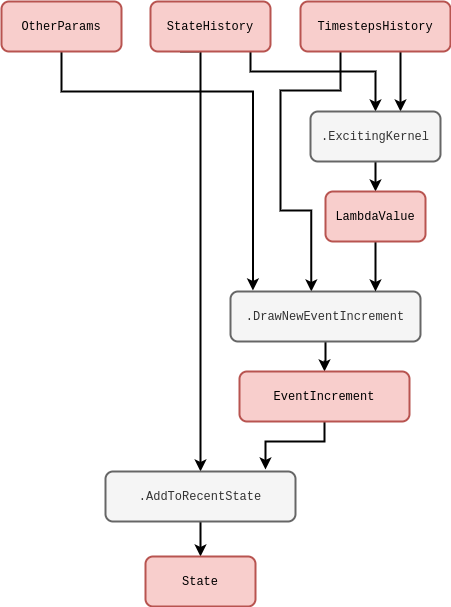
\includegraphics[width=9cm]{images/chapter-1-hawkes-process.drawio.png}
\caption{Schematic of code for a Hawkes process.}
\label{fig:hawkes-process}
\end{figure}

Note that this idea of integration kernels could also be applied back to our Wiener process. For example, another type of non-Markovian phenomenon that frequently arises across physical and life systems integrates the Wiener process history like so
%%
\begin{align}
S^{0}_{{\sf t}+1}(X',z,{\sf t}) &= W^0_{{\sf t}+1}-W^0_{\sf t}\\
S^{1}_{{\sf t}+1}(X',z,{\sf t}) &= u\sum^{{\sf t}}_{{\sf t}'=0}e^{-u[t({\sf t})-t({\sf t}')]} S^{0}_{{\sf t}'}\,,
\end{align}
%%
where $u$ is inversely proportional to the length of memory in continuous time.

\section{\sffamily Software design}

So we've proposed a computational formalism and then studied it in more detail to demonstrate that it can cope with a variety of different stochastic phenomena. Now we're ready to summarise what we want the stochadex software package to be able to do. But what's so complicated about Eq.~(\ref{eq:x-step-def})? Can't we just implement an iterative algorithm with a single function? It's true that the fundamental concept is very straightforward, but as we'll discuss in due course; the stochadex needs to have a lot of configurable features so that it's applicable in different situations. Ideally, the stochadex sampler should be designed to try and maintain a balance between performance and flexibility of utilisation.

If we begin with the obvious first set of criteria; we want to be able to freely configure the iteration function $F$ of Eq.~(\ref{eq:x-step-def}) and the timestep function $t$ of Eq.~(\ref{eq:t-steps-sum}) so that any process we want can be described. The point at which a simulation stops can also depend on some algorithm termination condition which the user should be able to specify up-front.

\begin{figure}[h]
\centering
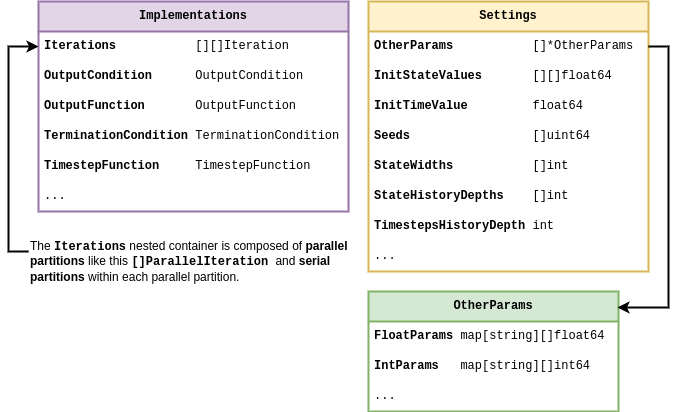
\includegraphics[width=13cm]{images/chapter-1-stochadex-data-types.drawio.png}
\caption{A relational summary of the configuration data types in the stochadex.}
\label{fig:data-types-design}
\end{figure}

Once the user has written the code to create these functions for the stochadex, we want to then be able to recall them in future only with configuration files while maintaining the possibility of changing their simulation run parameters. This flexibility should facilitate our uses for the simulation later in the book, and from this perspective it also makes sense that the parameters should include the random seed and initial state value.

The state history matrix $X$ should be configurable in terms of its number of rows --- what we'll call the `state width' --- and its number of columns --- what we'll call the `state history depth'. If we were to keep increasing the state width up to millions of elements or more, it's likely that on most machines the algorithm performance would grind to a halt when trying to iterate over the resulting $X$ within a single thread. Hence, before the algorithm or its performance in any more detail, we can pre-empt the requirement that $X$ should represented in computer memory by a set of partitioned matrices which are all capable of communicating to one-another downstream. In this paradigm, we'd like the user to be able to configure which state partitions are able to communicate with each other without having to write any new code.

For convenience, it seems sensible to also make the outputs from stochadex runs configurable. A user should be able to change the form of output that they want through, e.g., some specified function of $X$ at the time of outputting data. The times that the stochadex should output this data can also be decided by some user-specified condition so that the frequency of output is fully configurable as well. 

In summary, we've put together a schematic of configuration data types and their relationships in Fig.~\ref{fig:data-types-design}. In this diagram there is some indication of the data type that we propose to store each piece information in (in Go syntax), and the diagram as a whole should serve as a useful guide to the basic structure of configuration files for the stochadex.

It's clear that in order to simulate Eq.~(\ref{eq:x-step-def}), we need an interative algorithm which reapplies a user-specified function to the continually-updated history. But let's now return to the point we made earlier about how the performance of such an algorithm will depend on the size of the state history matrix $X$. The key bit of the algorithm design that isn't so straightforward is: how do we sucessfully split this state history up into separate partitions in memory while still enabling them to communicate effectively with each other? Other generalised simulation frameworks --- such as SimPy~\cite{simpy}, StoSpa~\cite{stospa} and FLAME GPU~\cite{flamegpu} --- have all approached this problem in different ways, and with different software architectures. 

In Fig.~\ref{fig:loop-design} we've illustrated what a loop involving separate state partitions looks like in the stochadex simulator. Each partition is handled by concurrently running execution threads of the same process, while a separate process may be used to handle the outputs from the algorithm. As the diagram shows, the main sequence of each loop iteration follows the pattern: 
%%
\begin{enumerate}
\item{The \texttt{PartitionCoordinator} requests more iterations from each state partition by sending an \texttt{IteratorInputMessage} to a concurrently running goroutine.}
\item{The \texttt{StateIterator} in each goroutine executes the iteration and stores the resulting state update in a variable.}
\item{Once all of the iterations have been completed, the \texttt{PartitionCoordinator} then requests each goroutine to update its relevant partition of the state history by sending another \texttt{IteratorInputMessage} to each.}
\end{enumerate}
%%
This pattern ensures that no partition has access to values in the state history which are out of sync with its current state in time, and hence prevents anachronisms from occuring in the overall state iteration. 

\begin{figure}[h]
\centering
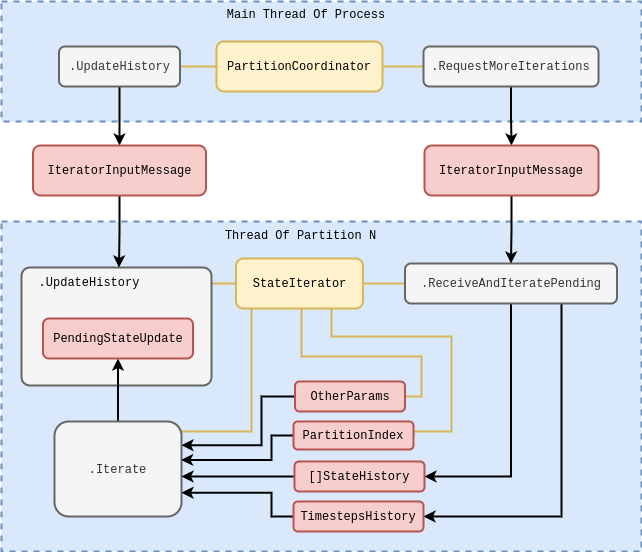
\includegraphics[width=13cm]{images/chapter-1-stochadex-loop.drawio.png}
\caption{Schematic for a step of the stochadex simulation algorithm.}
\label{fig:loop-design}
\end{figure}

It's also worth noting that while Fig.~\ref{fig:loop-design} illustrates only a single process; it's obviously true that we may run many of these whole diagrams at once to parallelise generating independent realisations of the simulation, if necessary.

As we stated at the beginning of this chapter: the full implementation of the stochadex can be found on GitHub by following this link: \href{https://github.com/umbralcalc/stochadex}{https://github.com/umbralcalc/stochadex}. Users can build the main binary executable of this repository and determine what configuration of the stochadex they would like to have through config at runtime (one can infer these configurations from Fig.~\ref{fig:data-types-design}). As Go is a statically typed language, this level of flexibility has been achieved using code templating proceeding runtime build and execution via \texttt{go run} `under-the-hood'. Users who find this particular execution pattern undesirable can also use all of the stochadex types, tools and methods as part of a standard library import.

In order to debug the simulation code and gain a more intuitive understanding of the outputs from a model as it is being developed, we have also written a lightweight frontend dashboard React~\cite{react} app in TypeScript to visualise any stochadex simulation as it is running. This dashboard can be launched by passing config at runtime to the main stochadex executable, and we have illustrated how all this fits together in a flowchart shown in Fig.~\ref{fig:stochadex-main}.

\begin{figure}[h]
\centering
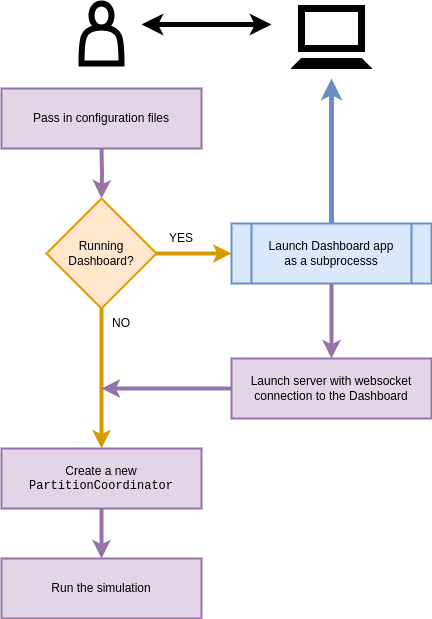
\includegraphics[width=9cm]{images/chapter-1-stochadex-main.drawio.png}
\caption{A diagram of the main stochadex binary executable.}
\label{fig:stochadex-main}
\end{figure}

